% Created 2014-06-13 Fri 12:06
\documentclass[bigger]{beamer}
\usepackage[utf8]{inputenc}
\usepackage[T1]{fontenc}
\usepackage{fixltx2e}
\usepackage{graphicx}
\usepackage{longtable}
\usepackage{float}
\usepackage{wrapfig}
\usepackage{soul}
\usepackage{textcomp}
\usepackage{marvosym}
\usepackage{wasysym}
\usepackage{latexsym}
\usepackage{amssymb}
\usepackage{hyperref}
\tolerance=1000
\mode<beamer>{\usetheme[compress]{Berlin}}
\usepackage{multirow}
\setbeamertemplate{footline}
  {%
    \begin{beamercolorbox}[colsep=1.5pt]{upper separation line foot}
    \end{beamercolorbox}
    \begin{beamercolorbox}[ht=2.5ex,dp=1.125ex,%
      leftskip=.3cm,rightskip=.3cm plus1fil]{author in head/foot}%
      \leavevmode{\usebeamerfont{author in head/foot}\insertshortauthor}%
      \hfill%
      {\usebeamerfont{institute in head/foot}\usebeamercolor[fg]{institute in head/foot}\insertshortinstitute}%
    \end{beamercolorbox}%
    \begin{beamercolorbox}[ht=2.5ex,dp=1.125ex,%
      leftskip=.3cm,rightskip=.3cm plus1fil]{title in head/foot}%
      {\usebeamerfont{title in head/foot}\insertshorttitle}%
      \hfill%
      {\usebeamerfont{frame number}\usebeamercolor[fg]{frame number}\insertframenumber~/~\inserttotalframenumber}
    \end{beamercolorbox}%
    \begin{beamercolorbox}[colsep=1.5pt]{lower separation line foot}
    \end{beamercolorbox}
  }
\makeatother


%----------------------------------------------------------------------
% Define useful commands
%----------------------------------------------------------------------

\newcommand{\eejj}{\ensuremath{eejj} }
\newcommand{\enujj}{\ensuremath{e\nu jj} }
\newcommand{\mumujj}{\ensuremath{\mu\mu jj} }
\newcommand{\munujj}{\ensuremath{\mu\nu jj} }
\newcommand{\emujj}{\ensuremath{e\mu jj} }
\newcommand{\zjets}{\ensuremath{\text{Z}^{0}}+jets }
\newcommand{\wjets}{\ensuremath{\text{W}^{\pm}}+jets }
\newcommand{\ttbar}{\ensuremath{t\bar{t}} }

\newcommand{\pt}{\ensuremath{p_{\text{T}}} }
\newcommand{\ST}{\ensuremath{S_{\text{T}}} }
\newcommand{\mee}{\ensuremath{m_{\text{ee}}} }
\newcommand{\mll}{\ensuremath{m_{\ell\ell}} }
\newcommand{\mej}{\ensuremath{m_{\text{ej}}} }
\newcommand{\mejmin}{\ensuremath{m_{\text{ej}}^{\text{min}}} }
\newcommand{\mejavg}{\ensuremath{m_{\text{ej}}^{\text{avg}}} }
% \newcommand{\mt}{\ensuremath{m_{\text{T, e}\nu}}}
\newcommand{\mtjnu}{\ensuremath{m_{\text{T, j}\nu}} }


\newcommand{\met}{\ensuremath{\not\!\!{E_{\text{T}}}} }
\newcommand{\mt}{\ensuremath{m_{\text{T, e}\nu}} }

%----------------------------------------------------------------------
% Define useful numbers
%----------------------------------------------------------------------

% Lumi info
\newcommand{\intLumi}{$19.6 \text{ fb}^{-1}$}

% MC scale factors
\newcommand{\enujjWJetsMonteCarloScaleFactor}{0.85 \pm 0.01 \text{ (stat)} \pm 0.01    \text{ (syst)}}
\newcommand{\enujjTTBarMonteCarloScaleFactor}{0.97 \pm 0.02 \text{ (stat)} \pm 0.01    \text{ (syst)}}
% \newcommand{\eejjZJetsMonteCarloScaleFactor} {0.97 \pm 0.01 \text{ (stat)} \pm 0.00004 \text{ (syst)}}
\newcommand{\eejjZJetsMonteCarloScaleFactor} {0.97 \pm 0.01 \text{ (stat)}}

\newcommand{\enujjWJetsMonteCarloScaleFactorMETRescaled}{0.95 \pm 0.02 \text{ (stat)} \pm 0.01 \text{ (syst)}}
\newcommand{\enujjTTBarMonteCarloScaleFactorMETRescaled}{1.07 \pm 0.03 \text{ (stat)} \pm 0.01 \text{ (syst)}}

\newcommand{\enujjWJetsMonteCarloScaleFactorMETandMTRescaled}{0.97 \pm 0.02 \text{ (stat)} \pm 0.01 \text{ (syst)}}
\newcommand{\enujjTTBarMonteCarloScaleFactorMETandMTRescaled}{1.08 \pm 0.03 \text{ (stat)} \pm 0.01 \text{ (syst)}}

\newcommand{\eejjZControlRegionContamination}{4\%}

% Electron scale factors
\newcommand{\electronRecoDataMCScaleFactor}{0.98}
\newcommand{\electronRecoDataMCScaleFactorRelUnc}{1.5}
\newcommand{\electronRecoDataMCScaleFactorSqr}{0.96}

% GEN-level cross-sections (not yet rescaled) 
\newcommand{\wjetsXSection}{37509.0 pb}
\newcommand{\zjetsXSection}{3503.71 pb}
\newcommand{\ttbarXSection}{234 pb}
\newcommand{\stopSChannelXSection}{5.55 pb}
\newcommand{\stopTChannelXSection}{87.1 pb}
\newcommand{\stopTWChannelXSection}{22.2 pb}
\newcommand{\wwXSection}{57.1 pb} % THESE NEED TO BE UPDATED!!!
\newcommand{\wzXSection}{32.3 pb} % THESE NEED TO BE UPDATED!!!
\newcommand{\zzXSection}{8.26 pb} % THESE NEED TO BE UPDATED!!!

% QCD contributions at limit of the analysis
\newcommand{\percentQCDatEEJJLimit}{1\%}
\newcommand{\percentQCDatENuJJLimit}{3\%}

% Closure test contamination
\newcommand{\percentContaminationClosureTest}{5\%}
\newcommand{\percentContaminationClosureTestFinal}{55\%}

% Closure test (low-ST) results
\newcommand{\closureTestLowSTPredicted}{13100}
\newcommand{\closureTestLowSTPredictedUnc}{400}
\newcommand{\closureTestLowSTObserved}{12100}
\newcommand{\closureTestLowSTObservedUnc}{400}
\newcommand{\closureTestLowSTRatio}{1.08}
\newcommand{\closureTestLowSTRatioUnc}{0.05}

% Closure test (mid-ST) results
\newcommand{\closureTestMidSTPredicted}{877}
\newcommand{\closureTestMidSTPredictedUnc}{46.7}
\newcommand{\closureTestMidSTObserved}{600}
\newcommand{\closureTestMidSTObservedUnc}{53}
\newcommand{\closureTestMidSTRatio}{1.46}
\newcommand{\closureTestMidSTRatioUnc}{0.15}

% QCD systematic uncertainty
\newcommand{\qcdSystematicUncertaintyPerEle}{30\%}
\newcommand{\qcdSystematicUncertaintyTwoEle}{60\%}

% TTbar (e-mu-jj) contamination
\newcommand{\emujjContamination}{2\%}
\newcommand{\emujjRecoScaleFactor}{0.974  \pm 0.011 \text{ (stat)}}

% mumujj/munujj scale factors for data-driven background
\newcommand{\mumujjRecoScaleFactor}{97.5 \pm 0.4 \text{ (stat)}}
\newcommand{\munujjRecoScaleFactor}{97.2 \pm 0.5 \text{ (stat)}}

% Shape uncertainties
\newcommand{\enujjWJetsShapeUncertainty}{5.92\%}
\newcommand{\enujjTTBarShapeUncertainty}{8.17\%}
\newcommand{\eejjZJetsShapeUncertainty}{8.70\%}

% EES uncertainties
\newcommand{\electronEnergyScaleUncBarrel}{0.4\%}
\newcommand{\electronEnergyScaleUncEndcap}{4.1\%}

% EER uncertainties
\newcommand{\electronEnergyResolutionUncBarrel}{1.006}
\newcommand{\electronEnergyResolutionUncEndcap}{1.015}

% lumi uncertainty
\newcommand{\lumiUncertainty}{2.6\%}

% limits
\newcommand{\eejjObservedLimit}{1005}
\newcommand{\eejjExpectedLimit}{1030}
\newcommand{\enujjObservedLimit}{845}
\newcommand{\enujjExpectedLimit}{890}

\newcommand{\enujjObservedLimitCombined}{845}
\newcommand{\enujjExpectedLimitCombined}{932}

\newcommand{\eejjObservedLimitNoSyst}{1010}
\newcommand{\eejjExpectedLimitNoSyst}{1030}
\newcommand{\enujjObservedLimitNoSyst}{850}
\newcommand{\enujjExpectedLimitNoSyst}{895}

\newcommand{\eejjObservedLimitMuon}{1015}
\newcommand{\eejjExpectedLimitMuon}{980}
\newcommand{\enujjObservedLimitMuon}{825}
\newcommand{\enujjExpectedLimitMuon}{890}


\newcommand{\lowBetaExpectedLimit}{790}
\newcommand{\lowBetaObservedLimit}{635}

\makeatletter
\newcommand\ChangeItemFont[3]{%
\renewcommand{\itemize}[1][]{%
  \beamer@ifempty{##1}{}{\def\beamer@defaultospec{#1}}%
  \ifnum \@itemdepth >2\relax\@toodeep\else
    \advance\@itemdepth\@ne
    \beamer@computepref\@itemdepth% sets \beameritemnestingprefix
    \usebeamerfont{itemize/enumerate \beameritemnestingprefix body}%
    \usebeamercolor[fg]{itemize/enumerate \beameritemnestingprefix body}%
    \usebeamertemplate{itemize/enumerate \beameritemnestingprefix body begin}%
    \list
      {\usebeamertemplate{itemize \beameritemnestingprefix item}}
      {\def\makelabel####1{%
          {%
            \hss\llap{{%
                \usebeamerfont*{itemize \beameritemnestingprefix item}%
                \usebeamercolor[fg]{itemize \beameritemnestingprefix item}####1}}%
          }%
        }%
  \ifnum\@itemdepth=1\relax
    #1%
  \else
  \ifnum\@itemdepth=2\relax
    #2%
  \else
  \ifnum\@itemdepth=3\relax
    #3%
  \fi%
  \fi%
  \fi%
  }
  \fi%
  \beamer@cramped%
  \raggedright%
  \beamer@firstlineitemizeunskip%
}}
\makeatother

\mode<beamer>{\usecolortheme{bear}}
\mode<beamer>{\titlegraphic{\includegraphics[width=0.2\textwidth]{brown-logo}}}
\institute[Brown University]{\inst{1} Brown University}
\providecommand{\alert}[1]{\textbf{#1}}

\title{HF Sourcing: \newline FFTs on Sourcing Data}
\author{Edmund Berry}
\date{Thursday, June 12, 2014}
\hypersetup{
  pdfkeywords={},
  pdfsubject={},
  pdfcreator={Emacs Org-mode version 7.8.11}}

\author[Edmund Berry]{\alert{Edmund Berry}\inst{1}}
\begin{document}

\maketitle


\section{Introduction}
\label{sec-1}
\subsection{Introduction}
\label{sec-1-1}
\begin{frame}
\frametitle{Fourier transforms reminder}
\label{sec-1-1-1}
\begin{itemize}

\item Fourier transform (FT) definition
\label{sec-1-1-1-1}%
\begin{itemize}

\item \(F(u) = \int_{-\infty}^{+\infty}f(t)e^{-2\pi i u t} dt\)
\label{sec-1-1-1-1-1}%
\end{itemize} % ends low level

\item FTs have real and imaginary components
\label{sec-1-1-1-2}%
\begin{itemize}

\item Real: \(\mathcal{R}(F)\)
\label{sec-1-1-1-2-1}%

\item Imaginary: \(\mathcal{I}(F)\)
\label{sec-1-1-1-2-2}%
\end{itemize} % ends low level

\item FTs have magnitude and phase in complex space:
\label{sec-1-1-1-3}%
\begin{itemize}

\item Magnitude: \(|F| = |\mathcal{R}(F)^{2} + \mathcal{I}(F)^{2}|^{1/2}\)
\label{sec-1-1-1-3-1}%

\item Phase: \(\phi(F) = \tan^{-1}\frac{\mathcal{R(F)}}{\mathcal{I(F)}}\)
\label{sec-1-1-1-3-2}%
\end{itemize} % ends low level
\end{itemize} % ends low level
\end{frame}
\begin{frame}
\frametitle{Method}
\label{sec-1-1-2}
\begin{itemize}

\item Two very simple steps
\label{sec-1-1-2-1}%
\begin{enumerate}
\item Use sine functions to test ROOT FFT software
\item Use ROOT FFT software to analyze sourcing data
\end{enumerate}

\item All of this code is on git:
\label{sec-1-1-2-2}%
\begin{enumerate}
\item \href{https://github.com/HCALPFG/HcalFFT/blob/master/FFT_tutorial.py}{\alert{Link to code}} for testing FFTs
\item \href{https://github.com/HCALPFG/HcalFFT/blob/master/FFT.py}{\alert{Link to code}} for running FFTs on sourcing data
\end{enumerate}
\end{itemize} % ends low level
\end{frame}
\section{FFT test on sine functions}
\label{sec-2}
\subsection{FFT test on sine functions}
\label{sec-2-1}
\begin{frame}
\frametitle{FFT test on sine functions}
\label{sec-2-1-1}
%% Figure
\label{sec-2-1-1-1}

\centering
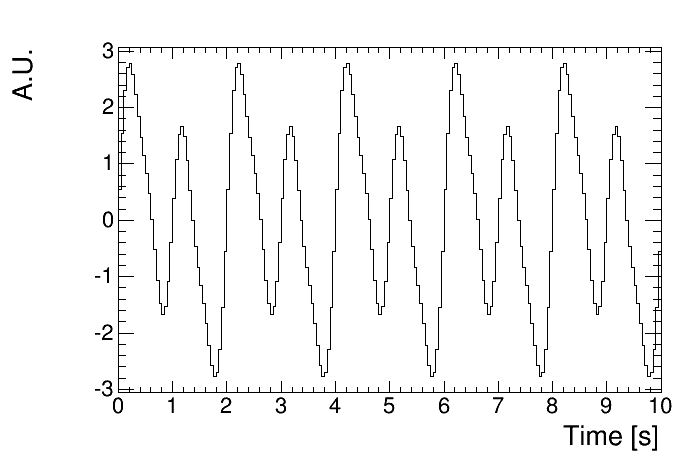
\includegraphics[width=0.6\textwidth]{fig/tutorial_original_histogram.png}
\begin{itemize}

\item Fill a histogram using linear combo of sine functions:
\label{sec-2-1-1-2}%
\begin{itemize}

\item \(f(t) = \sum_{i = 0}^3 A_{i} \cdot \sin (2\pi \cdot f_{i} \cdot t)\)
\label{sec-2-1-1-2-1}%

\item \(A_{i} = \{1.0, 2.0, 0.5\}\) [A.U.]
\label{sec-2-1-1-2-2}%

\item \(f_{i} = \{0.5, 1.0, 2.0\}\) [Hz]
\label{sec-2-1-1-2-3}%
\end{itemize} % ends low level
\end{itemize} % ends low level
\end{frame}
\begin{frame}
\frametitle{Look at magnitude of FFT}
\label{sec-2-1-2}
%% Figure
\label{sec-2-1-2-1}

\centering
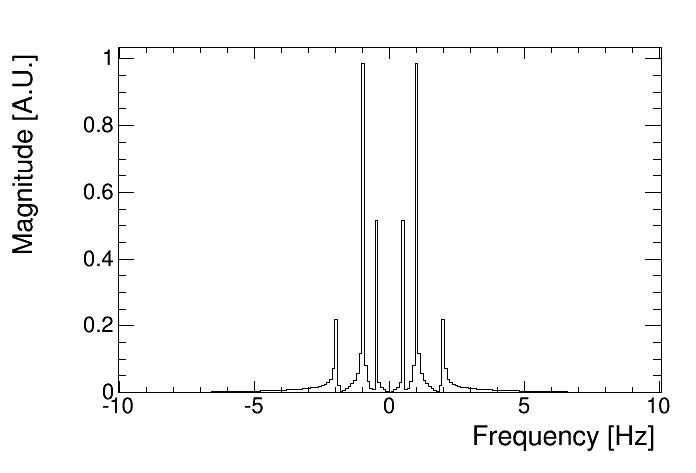
\includegraphics[width=0.6\textwidth]{fig/tutorial_FFT_magnitude.png}
\begin{itemize}

\item Recall original linear combo of sine functions:
\label{sec-2-1-2-2}%
\begin{itemize}

\item \(f(t) = \sum_{i = 0}^3 A_{i} \cdot \sin (2\pi \cdot f_{i} \cdot t)\)
\label{sec-2-1-2-2-1}%

\item \(A_{i} = \{1.0, 2.0, 0.5\}\) [A.U.]
\label{sec-2-1-2-2-2}%

\item \(f_{i} = \{0.5, 1.0, 2.0\}\) [Hz]
\label{sec-2-1-2-2-3}%
\end{itemize} % ends low level
\end{itemize} % ends low level
\end{frame}
\begin{frame}
\frametitle{Look at magnitude of FFT (left side of function)}
\label{sec-2-1-3}
%% Figure
\label{sec-2-1-3-1}

\centering
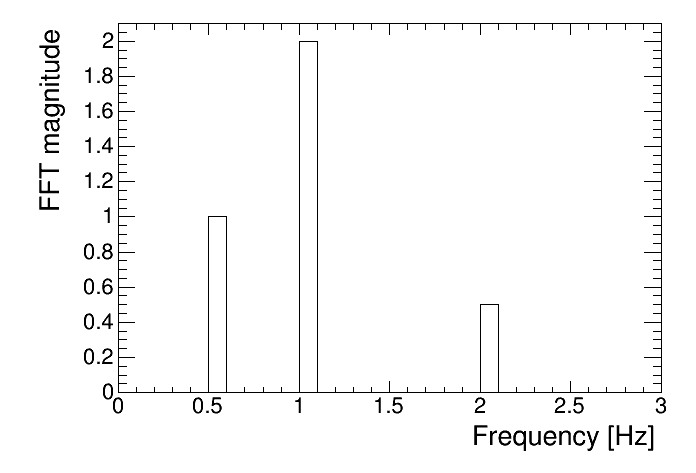
\includegraphics[width=0.6\textwidth]{fig/tutorial_FFT_magnitude_scaled.png}
\begin{itemize}

\item Magnitude (even function) returns \(A_{i}\) and \(f_{i}\)
\label{sec-2-1-3-2}%
\begin{itemize}

\item \(f(t) = \sum_{i = 0}^3 A_{i} \cdot \sin (2\pi \cdot f_{i} \cdot t)\)
\label{sec-2-1-3-2-1}%

\item \(A_{i} = \{1.0, 2.0, 0.5\}\) [A.U.]
\label{sec-2-1-3-2-2}%

\item \(f_{i} = \{0.5, 1.0, 2.0\}\) [Hz]
\label{sec-2-1-3-2-3}%
\end{itemize} % ends low level
\end{itemize} % ends low level
\end{frame}
\begin{frame}
\frametitle{Look at phase of FFT}
\label{sec-2-1-4}
%% Figure
\label{sec-2-1-4-1}

\centering
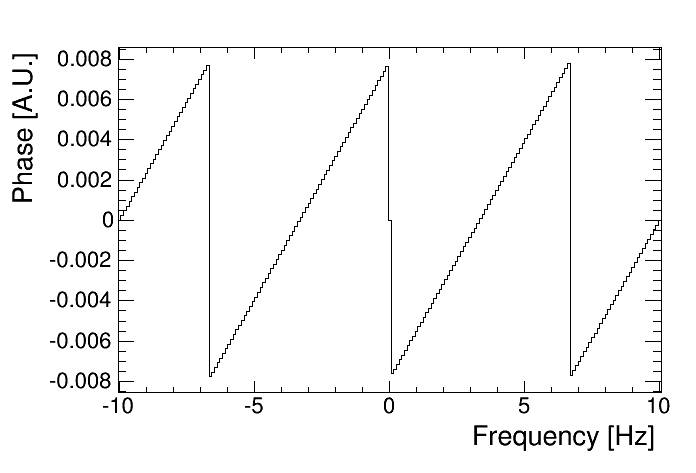
\includegraphics[width=0.6\textwidth]{fig/tutorial_FFT_phase.png}
\begin{itemize}

\item Phase information not useful for our purposes\ldots{}
\label{sec-2-1-4-2}%
\begin{itemize}

\item \(f(t) = \sum_{i = 0}^3 A_{i} \cdot \sin (2\pi \cdot f_{i} \cdot t)\)
\label{sec-2-1-4-2-1}%

\item \(A_{i} = \{1.0, 2.0, 0.5\}\) [A.U.]
\label{sec-2-1-4-2-2}%

\item \(f_{i} = \{0.5, 1.0, 2.0\}\) [Hz]
\label{sec-2-1-4-2-3}%
\end{itemize} % ends low level
\end{itemize} % ends low level
\end{frame}
\begin{frame}
\frametitle{Conclusion of test:}
\label{sec-2-1-5}
\begin{itemize}

\item Can use ROOT FFT software
\label{sec-2-1-5-1}%

\item ROOT FFT software can reconstruct parameters of sines
\label{sec-2-1-5-2}%
\begin{itemize}

\item FT magnitude contains useful information for analysis
\label{sec-2-1-5-2-1}%

\item FT phase not useful for this analysis (?)
\label{sec-2-1-5-2-2}%

\item Can use FT phase to reconstruct original function (inverse FFT)
\label{sec-2-1-5-2-3}%
\end{itemize} % ends low level

\item Ready to try sourcing data
\label{sec-2-1-5-3}%
\end{itemize} % ends low level
\end{frame}
\section{FFTs on data}
\label{sec-3}
\subsection{FFTs on data}
\label{sec-3-1}
\begin{frame}
\frametitle{Look at sourcing data}
\label{sec-3-1-1}
\begin{itemize}

\item histogram name:\\
\label{sec-3-1-1-1}%
``\texttt{HFP13\_ETA38\_PHI25\_T10\_SRCTUBE\_} \newline{}
\texttt{Ieta38\_Iphi25\_Depth2}  \newline{}
\texttt{Run 221509reelPosition}''

\item $x$-axis: Reel [mm]
\label{sec-3-1-1-2}%

\item $y$-axis: Histogram mean [linear ADC]
\label{sec-3-1-1-3}%
\end{itemize} % ends low level
\end{frame}
\begin{frame}
\frametitle{Look at sourcing data: full range of reel vals}
\label{sec-3-1-2}
%% Figure
\label{sec-3-1-2-1}

\centering
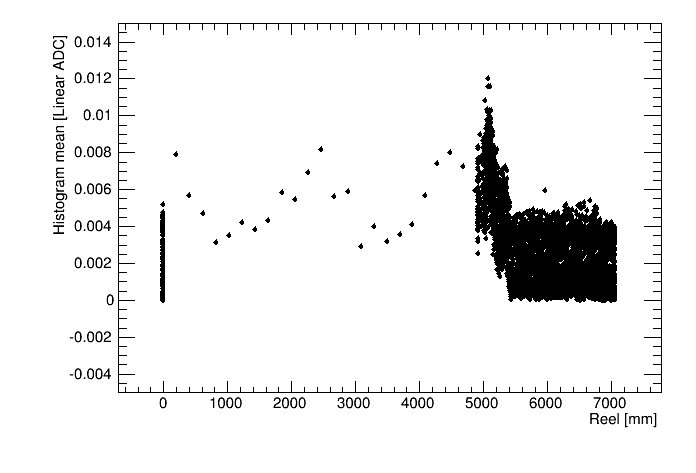
\includegraphics[width=0.6\textwidth]{fig/sourcing_unzoomed_plot.png}
\begin{itemize}

\item Next: focus on \(\text{reel } \epsilon \text{ } [5800, 6800] \text{ [mm]}\), where amplitude is stable
\label{sec-3-1-2-2}%
\end{itemize} % ends low level
\end{frame}
\begin{frame}
\frametitle{Look at sourcing data: zoomed reel vals (TGraph)}
\label{sec-3-1-3}
%% Figure
\label{sec-3-1-3-1}

\centering
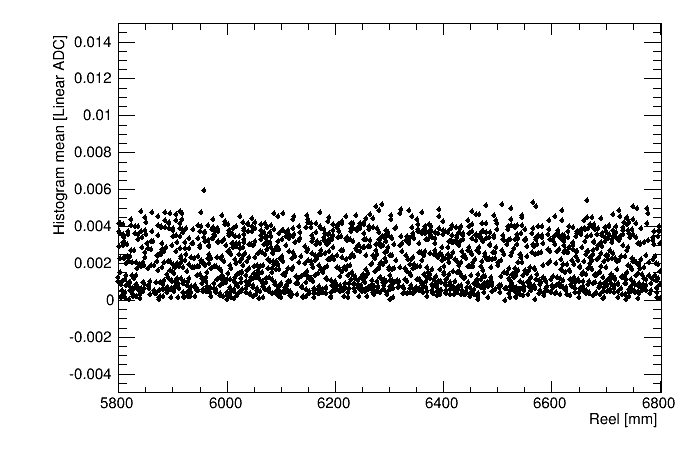
\includegraphics[width=0.6\textwidth]{fig/sourcing_zoomed_plot.png}
\begin{itemize}

\item This looks stable.  We can do our FFT on this data.
\label{sec-3-1-3-2}%

\item Next: zoom in even further \(([6000,6050])\) to see what frequency we suspect naively
\label{sec-3-1-3-3}%
\end{itemize} % ends low level
\end{frame}
\begin{frame}
\frametitle{Look at sourcing data: zoomed reel vals (TGraph)}
\label{sec-3-1-4}
%% Figure
\label{sec-3-1-4-1}

\centering
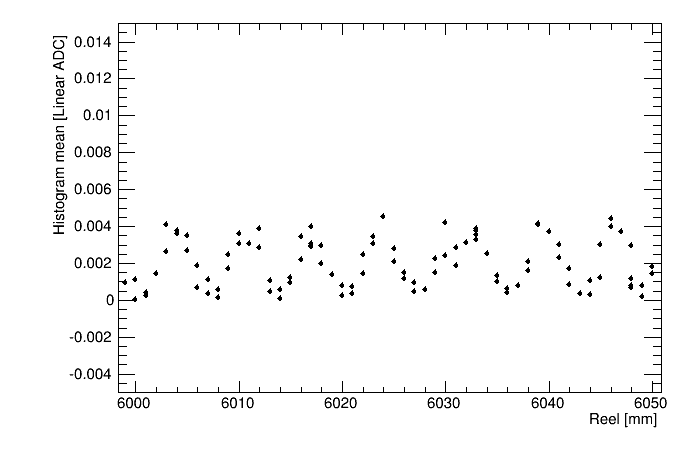
\includegraphics[width=0.6\textwidth]{fig/sourcing_very_zoomed_plot.png}
\begin{itemize}

\item 7 periods in 50mm:
\label{sec-3-1-4-2}%
\begin{itemize}

\item \(T = 50 \text{ [mm]}/ 7 = 7.14 \text{ [mm]} \)
\label{sec-3-1-4-2-1}%

\item \(f = 1/T = 0.14 \text{ [1/mm]}\)
\label{sec-3-1-4-2-2}%
\end{itemize} % ends low level

\item Only a naive guess for the frequency!
\label{sec-3-1-4-3}%
\end{itemize} % ends low level
\end{frame}
\begin{frame}
\frametitle{Look at sourcing data: zoomed reel vals (TH1F)}
\label{sec-3-1-5}
%% Figure
\label{sec-3-1-5-1}

\centering
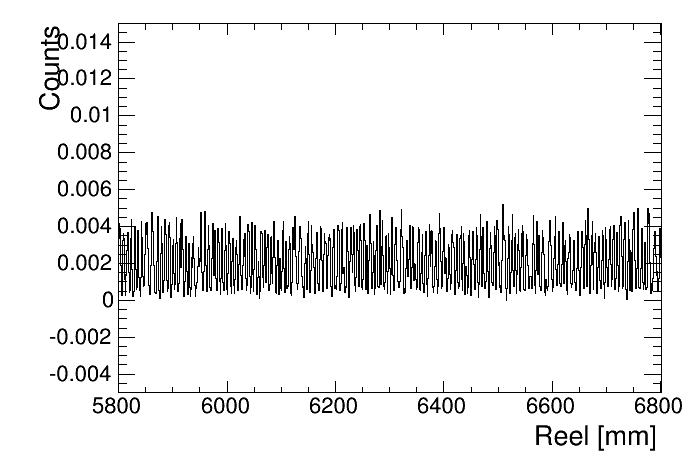
\includegraphics[width=0.6\textwidth]{fig/original_histogram.png}
\begin{itemize}

\item Now make a histogram from the TGraph (result above)
\label{sec-3-1-5-2}%
\begin{itemize}

\item If multiple points in TGraph have the same $x$-value, use their mean $y$-value on $y$-axis for histogram
\label{sec-3-1-5-2-1}%
\end{itemize} % ends low level

\item Next: do FFT on this histogram
\label{sec-3-1-5-3}%
\end{itemize} % ends low level
\end{frame}
\begin{frame}
\frametitle{Look at sourcing data: FFT magnitude}
\label{sec-3-1-6}
%% Figure
\label{sec-3-1-6-1}

\centering
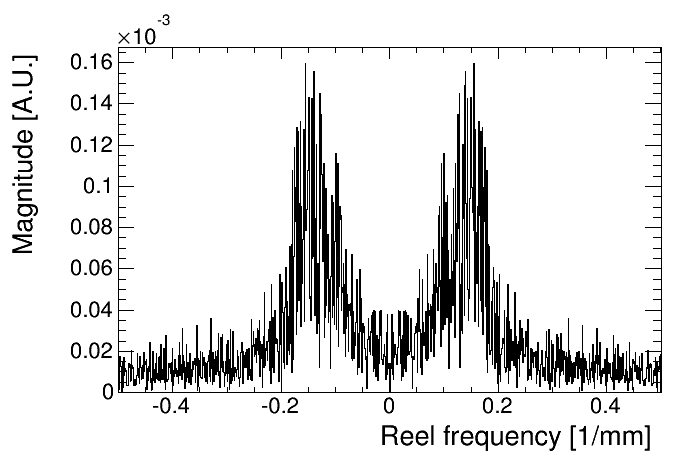
\includegraphics[width=0.6\textwidth]{fig/FFT_magnitude.png}
\begin{itemize}

\item Magnitude at zero is very large, because $y$-values of the original histogram are not centered at zero
\label{sec-3-1-6-2}%

\item Next: remove bin at Frequency = 0
\label{sec-3-1-6-3}%
\end{itemize} % ends low level
\end{frame}
\begin{frame}
\frametitle{Look at sourcing data: FFT magnitude, no first bin}
\label{sec-3-1-7}
%% Figure
\label{sec-3-1-7-1}

\centering
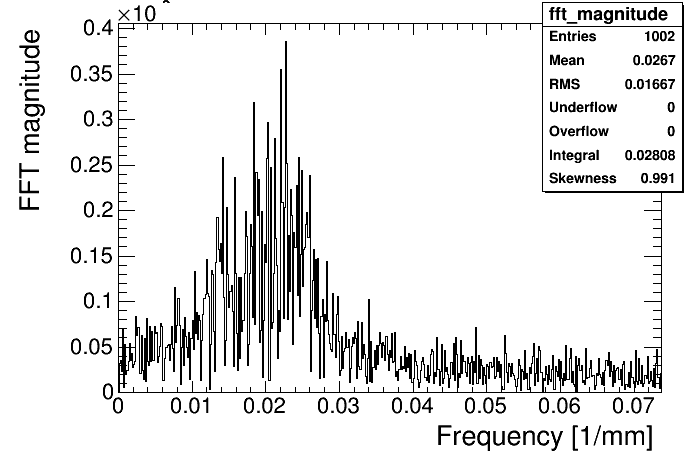
\includegraphics[width=0.6\textwidth]{fig/FFT_magnitude_zeroFirstBin.png}
\begin{itemize}

\item Now we can see the structure of the FFT magnitude
\label{sec-3-1-7-2}%

\item Next: consider only the upper ``half'' of the magnitude's range
\label{sec-3-1-7-3}%
\end{itemize} % ends low level
\end{frame}
\begin{frame}
\frametitle{Look at sourcing data: FFT magnitude, upper half}
\label{sec-3-1-8}
%% Figure
\label{sec-3-1-8-1}

\centering
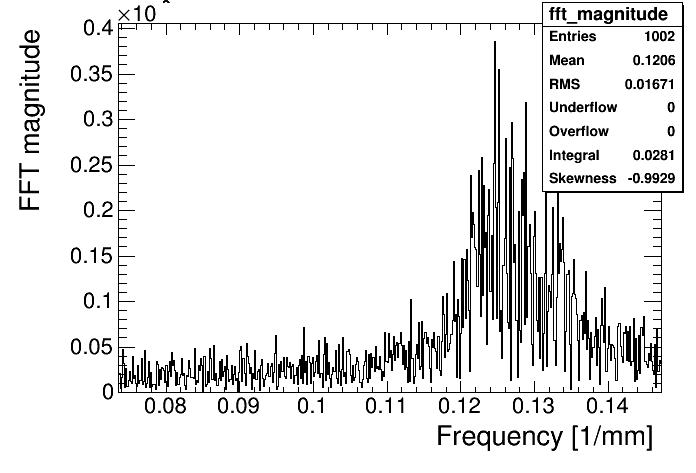
\includegraphics[width=0.6\textwidth]{fig/FFT_magnitude_zeroFirstBin_upperHalf.png}
\begin{itemize}

\item FFT magnitude peaks between ``reel frequency''\\
\label{sec-3-1-8-2}%
(in [1/mm]) of 0.12 and 0.13 

\item Roughly matches our naive guess (0.14)
\label{sec-3-1-8-3}%
\end{itemize} % ends low level
\end{frame}
\section{Conclusion}
\label{sec-4}
\subsection{Conclusion}
\label{sec-4-1}
\begin{frame}
\frametitle{Conclusion}
\label{sec-4-1-1}
\begin{itemize}

\item We can use ROOT software to do FFTs
\label{sec-4-1-1-1}%
\begin{itemize}

\item Tests done on sine waves in time / frequency space
\label{sec-4-1-1-1-1}%

\item Prelim. results on data in reel / ``reel frequency'' space
\label{sec-4-1-1-1-2}%
\end{itemize} % ends low level

\item Prelim. results show peak in ``reel frequency''
\label{sec-4-1-1-2}%
\begin{itemize}

\item Around 0.12 - 0.13 [1/mm]
\label{sec-4-1-1-2-1}%
\end{itemize} % ends low level

\item Would be nice to repeat the study on sourcing data in time (OrN)
\label{sec-4-1-1-3}%
\begin{itemize}

\item Need plots for this
\label{sec-4-1-1-3-1}%
\end{itemize} % ends low level
\end{itemize} % ends low level
\end{frame}

\end{document}
